\documentclass{article}
\usepackage{graphicx}
\usepackage{amsmath}
\DeclareMathOperator{\floor}{floor}
\begin{document}

\begin{figure}[ht!]
\centering
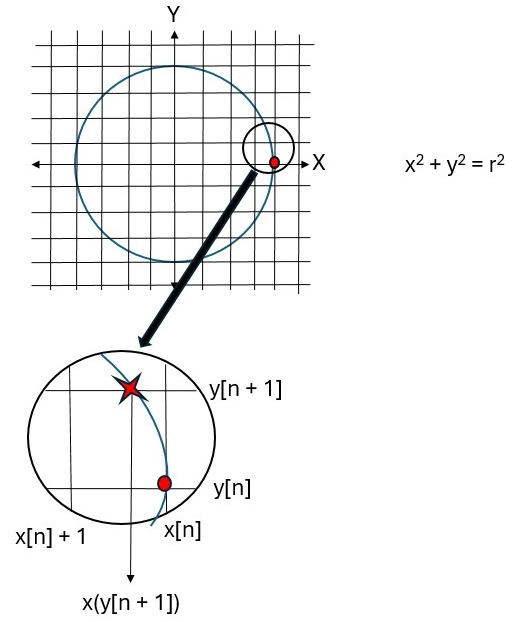
\includegraphics[width=90mm]{Circle Rasterization.jpg}
\caption{Circle Rasterization Algorithm \label{overflow}}
\end{figure}



\underline{\textbf{First Octant Rasterization Algorithm:}} \\
\begin{enumerate}
    \item \underline{Set Initial Values:} 
          \begin{align*}
                x[0] = r, \quad y[0] = 0 
            \end{align*}
    \item \underline{for $n = 0 \rightarrow N - 1$:} \\
          \begin{align*}
            &y[n + 1] = y[n] + 1 \\ \\
            &x[n + 1] = \begin{cases}
                            x[n] \quad \ \ \ , \quad x[n] - x\Big(y[n + 1]\Big) < 0.5 \\ \\
                            x[n] - 1 \ , \quad x[n] - x\Big(y[n + 1]\Big) \geq 0.5
                          \end{cases}
      \end{align*}
\end{enumerate}

\underline{\textbf{Initial Mathematics:}}
\begin{align*}
    &\quad \ \ x^{2} + y^{2} = r^{2} \\ \\
    &\Rightarrow x^{2} = r^{2} - y^{2} \\ \\
    &\Rightarrow x(y) = \pm\sqrt{r^{2} - y^{2}} \\ \\
    &\quad \quad \quad \ \ = \begin{cases}
                                \ \ \sqrt{r^{2} - y^{2}}, \quad y \geq 0 \quad \ \ \big(\text{Top Half-Circle}\big) \\ \\
                                -\sqrt{r^{2} - y^{2}}, \quad y < 0 \quad \big(\text{Bottom Half-Circle}\big) \\ \\ 
                               \end{cases} \\ \\
    &\quad \quad \quad \ \ = \sqrt{r^{2} - y^{2}} \quad \big(\text{Only need Top Half-Circle for Rasterization}\big) \\ \\
    &\Rightarrow \frac{dx(y)}{dy} = \frac{-y}{\sqrt{r^{2} - y^{2}}} \\ \\
\end{align*}

\underline{\textbf{Incremental Axis Calculation:}}
\begin{align*}
    &\quad \ \ y[n + 1] = y[n] + 1 \\ \\
    &\Rightarrow y[n] = y[n - 1] + 1 \\ \\
    &\quad \quad \quad \ = y[n - 2] + 2 \\ \\
    &\quad \quad \quad \ = y[n - n] + n \\ \\
    &\quad \quad \quad \ = n
\end{align*}

\underline{\textbf{Orthogonal Axis Calculation:}}
\begin{align*}
    x\Big(y[n + 1]\Big) &= \sqrt{r^{2} - y^{2}[n + 1]} \\ \\
                        &= \sqrt{r^{2} - \big(n + 1\big)^{2}} \\ \\
\end{align*}

\underline{\textbf{Decision Optimization:}}
\begin{align*}
    &\quad \quad \quad \ \ x[n] - x\Big(y[n + 1]\Big) \geq 0.5 \\ \\
    &\quad \quad \Rightarrow 2x[n] - 2x\Big(y[n + 1]\Big) \geq 1 \quad \big(\text{Integer Bitshift Modification}\big) \\ \\
    &\quad \quad \Rightarrow 2x[n] - 2\sqrt{r^{2} - \big(n + 1\big)^{2}} \geq 1 \\ \\
    &\quad \quad \Rightarrow 2\sqrt{r^{2} - \big(n + 1\big)^{2}} \leq 2x[n] - 1 \\ \\
    &\quad \quad \Rightarrow 4\Big(r^{2} - \big(n + 1\big)^{2}\Big) \leq \Big(2x[n] - 1\Big)^{2} \quad \big(\text{Only possible since we remain in first quadrant}\big) \\ \\
    &\quad \quad \Rightarrow 4\Big(x^{2}[n] - x[n] + n^{2} + 2n\Big) \geq \tau, \quad \tau \equiv 4r^{2} - 5 \\ \\
\end{align*}

\underline{\textbf{Number of elements:}}
\begin{align*}
    &\quad \quad \frac{dx\Big(y[N - 1]\Big)}{dy} \leq -1 \quad \big(\text{Second-to-last element should satisfy this condition}\big) \\ \\
    &\Rightarrow \frac{-y[N - 1]}{\sqrt{r^{2} - y^{2}[N - 1]}} \leq -1 \\ \\
    &\Rightarrow \frac{-(N - 1)}{\sqrt{r^{2} - \big(N - 1\big)^{2}}} \leq -1 \\ \\
    &\Rightarrow N - 1 \leq \frac{r}{\sqrt{2}} \\ \\
    &\Rightarrow N = \floor\Bigg(\frac{r}{\sqrt{2}}\Bigg) + 1\\ \\
\end{align*}

\underline{\textbf{Final First Octant Rasterization Algorithm:}} \\
\begin{enumerate}
    \item \underline{Set Initial Values:} 
          \begin{align*}
                &x[0] = r, \quad y[0] = 0 \\ \\
                &N = \floor\Bigg(\frac{r}{\sqrt{2}}\Bigg) \\ \\
                &\tau = 4r^{2} - 5
            \end{align*}
    \item \underline{for $n = 0 \rightarrow N - 1$:} \\
          \begin{align*}
            &y[n + 1] = y[n] + 1 \\ \\
            &x[n + 1] = x[n] - d, \quad d \equiv \begin{cases}
                                                     0 \ , \quad 4\Big(x^{2}[n] - x[n] + n^{2} + 2n\Big) < \tau \\ \\
                                                     1 \ , \quad 4\Big(x^{2}[n] - x[n] + n^{2} + 2n\Big) \geq \tau
                                                   \end{cases}
      \end{align*}
\end{enumerate}

\end{document}
